\documentclass[12pt]{article}

\usepackage[utf8]{inputenc}
\usepackage{latexsym,amsfonts,amssymb,amsthm,amsmath}
\usepackage{tikz}
\usepackage{stanli}
\usetikzlibrary{calc,through}
\usepackage{multicol}
\usepackage{geometry} 
\usepackage{enumitem}


\setlength{\parindent}{0in}
\setlength{\oddsidemargin}{-0.25in}
\setlength{\textwidth}{7in}
\setlength{\textheight}{9.3in}
\setlength{\topmargin}{-1in}
\setlength{\headheight}{18pt}

\newcommand\blfootnote[1]{%
  \begingroup
  \renewcommand\thefootnote{}\footnote{#1}%
  \addtocounter{footnote}{-1}%
  \endgroup
}

\title{ME473 Dynamic Finite Element Analysis Mini-Project}
\author{Stefano Burzio}
\date{}

\begin{document}
\noindent ME473 - Dynamic finite element analysis of structures\hfill EPFL\\
Stefano Burzio \hfill 2025\\
\vspace{0.3cm}

\hspace*{\fill}\textbf{\Large Mini-project 3}\hspace*{\fill}
\begin{center}
  \textbf{\Large Natural frequencies and mode shapes of a square plate}
\end{center}

\hrulefill
\vspace{0.3cm}
\newline
{Project organization:}
\vspace{0.2cm}
\newline
\begin{minipage}[t]{0.38\textwidth}
  \begin{itemize}[itemsep=0.005cm]
    \item Groups: 3 to 5 students
    \item 20\% of final grade
    \item Pdf report: maximum 10 pages
  \end{itemize}
\end{minipage}
\hfill
\begin{minipage}[t]{0.58\textwidth}
  \begin{itemize}[itemsep=0.005cm]
    \item Programming language: Matlab
    \item Submission: 1 June, 2025
    \item Total workload:  40h (approx. 10h per student)
  \end{itemize}
\end{minipage}
\vspace{0.3cm}

\hrulefill
\vspace{0.3cm}

\begin{center}
  \begin{tikzpicture}
    \point{a}{0}{-0.3};
    \point{b}{2.5}{-0.3};
    \point{c}{5}{-0.3};
    \point{d}{6}{0.7};
    \point{e}{7}{1.7};
    \support{1}{a};
    \support{1}{b};
    \support{1}{c};
    \support{1}{d};
    \support{1}{e};
    % Axes
    \draw[ultra thin,-latex] (-0.5,-0.65) -- (2.7,2.55) node[above] {$y$};
    % Draw the rectangle (domain)
    \filldraw[fill=gray!40, draw=black,thick]  (0,0) -- (5,0) -- (7,2) -- (2,2) -- cycle;
    \filldraw[fill=gray!40, draw=black,thick]  (0,0) -- (5,0) -- (5,-0.3) -- (0,-0.3) -- cycle;
    \filldraw[fill=gray!40, draw=black,thick]  (5,0) -- (7,2) -- (7,1.7) -- (5,-0.3) --cycle;
    % Axes
    \draw[ultra thin,-latex] (-0.7,-0.15) -- (7,-0.15) node[right] {$x$};
    % Labels
    \draw[ultra thin] (5.2,1) -- (7,3) node[right]{$\ell,h,E, \nu, \rho$};
  \end{tikzpicture}
\end{center}

\begin{enumerate}
  \item[a)] Model, using the finite element method, a square, isotropic, thin plate that is simply supported along all four edges using two $n \times n$ meshes, one using AMC plate bending elements and the second using CR plate bending elements. The geometrical and material properties of the plate are given as:
        \begin{itemize}
          \item length of the edge \(\ell=0.5\) m,
          \item thickness \(h=0.005\) m,
          \item elasticity modulus \(E=210\) GPa,
          \item Poisson's ratio $\nu=0.3$,
          \item density \(\rho=7850\) kg/m$^3$.
        \end{itemize}

  \item[b)] Compute the approximate first natural frequencies and corresponding mode shapes of the plate for discretizations with $2 \times 2$, $4 \times 4$, $8 \times 8$, and $16 \times 16$ elements. Discuss the results, compare them against exact analytical frequencies, and evaluate the convergence behavior of the numerical predictions.

  \item[c)] Investigate the effect of changing the span/thickness ratio from $\ell/h=100$ to $\ell/h=10$ on the accuracy of the lowest frequency of a simply supported square plate computed using AMC or CR elements. Compare the results obtained using a thin plate formulation with the exact one and with the one obtained from a thick plate model.
\end{enumerate}

\end{document}
